%----------------------------------------------------------------------------------------
%	PACKAGES AND OTHER DOCUMENT CONFIGURATIONS
%----------------------------------------------------------------------------------------

\documentclass[landscape,a0paper,fontscale=0.4]{baposter} % Adjust the font scale/size here

\usepackage{calc}
\usepackage{relsize}   % For \smaller
%\usepackage{multirow}
%\usepackage{rotating}
%\usepackage{bm}
\usepackage{url}       % For \url

\usepackage{graphicx}
%\usepackage{subcaption} % For floating figures

\usepackage{multicol} % Required for multiple columns
%\usepackage{wrapfig}
\setlength{\columnsep}{1.5em} % Slightly increase the space between columns
\setlength{\columnseprule}{0mm} % No horizontal rule between columns

\usepackage{tikz} % Required for flow chart
\usetikzlibrary{calc}

%\usepackage{times}
%\usepackage{helvet}
%\usepackage{bookman}
\usepackage{palatino}

%%% Global Settings %%%%%%%%%%%%%%%%%%%%%%%%%%%%%%%%%%%%%%%%%%%%%%%%%%%%%%%%%%%

\graphicspath{{images/}{draw.io/}}	% Root directory of the pictures
%\tracingstats=2			% Enabled LaTeX logging with conditionals

%%%%%%%%%%%%%%%%%%%%%%%%%%%%%%%%%%%%%%%%%%%%%%%%%%%%%%%%%%%%%%%%%%%%%%%%%%%%%%%%
% Save space in lists. Use this after the opening of the list
%%%%%%%%%%%%%%%%%%%%%%%%%%%%%%%%%%%%%%%%%%%%%%%%%%%%%%%%%%%%%%%%%%%%%%%%%%%%%%%%
\newcommand{\compresslist}{%
\setlength{\itemsep}{1pt}%
\setlength{\parskip}{0pt}%
\setlength{\parsep}{0pt}%
}

%%%%%%%%%%%%%%%%%%%%%%%%%%%%%%%%%%%%%%%%%%%%%%%%%%%%%%%%%%%%%%%%%%%%%%%%%%%%%%
%%% Begin of Document
%%%%%%%%%%%%%%%%%%%%%%%%%%%%%%%%%%%%%%%%%%%%%%%%%%%%%%%%%%%%%%%%%%%%%%%%%%%%%%

\begin{document}

%%%%%%%%%%%%%%%%%%%%%%%%%%%%%%%%%%%%%%%%%%%%%%%%%%%%%%%%%%%%%%%%%%%%%%%%%%%%%%
%%% Here starts the poster
%%%---------------------------------------------------------------------------
%%% Format it to your taste with the options
%%%%%%%%%%%%%%%%%%%%%%%%%%%%%%%%%%%%%%%%%%%%%%%%%%%%%%%%%%%%%%%%%%%%%%%%%%%%%%
% Define some colors

%\definecolor{lightblue}{cmyk}{0.83,0.24,0,0.12}
\definecolor{lightblue}{rgb}{0.145,0.6666,1}
%\definecolor{copernicusred}{rgb}{0.50,0.14,0.22}

%%
\begin{poster}%
  % Poster Options
  {
  % Show grid to help with alignment
  grid=false,
  % Number of columns
  columns=4,
  % Column spacing
  colspacing=1em,
  % Color style
  bgColorOne=white, % Background color for the gradient on the left side of the poster
  bgColorTwo=white, % Background color for the gradient on the right side of the poster
  borderColor=lightblue, % Border color
  headerColorOne=black, % Background color for the header in the content boxes (left side)
  headerColorTwo=lightblue, % Background color for the header in the content boxes (right side)
  headerFontColor=white, % Text color for the header text in the content boxes
  boxColorOne=white, % Background color of the content boxes
  boxColorTwo=lightblue,
  % Format of textbox
  textborder=roundedleft,
  % Format of text header
  eyecatcher=false, % Set to false for ignoring the left logo in the title and move the title left
  headerborder=closed, % Adds a border around the header of content boxes
  headerheight=0.10\textheight, % Height of the header
  headershape=roundedright, % Specify the rounded corner in the content box headers
  headershade=shadelr,
  headerfont=\Large\bf\textsf, %Sans Serif
  % textfont={\setlength{\parindent}{1.5em}},
  % boxshade=plain,
  % background=shade-tb,
  % background=plain,
  linewidth=2pt
  }
%%% Eye Cacther %%%%%%%%%%%%%%%%%%%%%%%%%%%%%%%%%%%%%%%%%%%%%%%%%%%%%%%%%%%%%%%
  {} % No eye catcher for this poster. If an eye catcher is present, the title is centered between eye-catcher and logo.
  % {
  %     
\includegraphics[width=10em]{copernicus-logo}
  %     \includegraphics[width=12em]{c3s-logo}
  % }
%%% Title %%%%%%%%%%%%%%%%%%%%%%%%%%%%%%%%%%%%%%%%%%%%%%%%%%%%%%%%%%%%%%%%%%%%%
  {\sf %Sans Serif
  Web Processing Services for Copernicus Climate Change Service
  }
%%% Authors %%%%%%%%%%%%%%%%%%%%%%%%%%%%%%%%%%%%%%%%%%%%%%%%%%%%%%%%%%%%%%%%%%%
  {\sf %Sans Serif
    C. Ehbrecht\footnotemark[2], A. Stephens\footnotemark[1], S. Kindermann\footnotemark[2], S. Denvil\footnotemark[3]\\
    {\smaller Centre for Environmental Data Analysis (CEDA)\footnotemark[1],
    German Climate Compute Centre (DKRZ)\footnotemark[2],
    Institut Pierre Simon Laplace (IPSL)\footnotemark[3]}\hspace{7em}
    \includegraphics[width=3em]{egu-logo} Vienna, 2018
  }
%%% Logo %%%%%%%%%%%%%%%%%%%%%%%%%%%%%%%%%%%%%%%%%%%%%%%%%%%%%%%%%%%%%%%%%%%%%%
  {
    \begin{minipage}{30em}
      \hfill
      
\includegraphics[width=10em]{copernicus-logo}
      \includegraphics[width=12em]{c3s-logo}
    \end{minipage}
  }

%%%%%%%%%%%%%%%%%%%%%%%%%%%%%%%%%%%%%%%%%%%%%%%%%%%%%%%%%%%%%%%%%%%%%%%%%%%%%%
%%% Now define the boxes that make up the poster
%%%---------------------------------------------------------------------------
%%% Each box has a name and can be placed absolutely or relatively.
%%% The only inconvenience is that you can only specify a relative position
%%% towards an already declared box. So if you have a box attached to the
%%% bottom, one to the top and a third one which should be in between, you
%%% have to specify the top and bottom boxes before you specify the middle
%%% box.
%%%%%%%%%%%%%%%%%%%%%%%%%%%%%%%%%%%%%%%%%%%%%%%%%%%%%%%%%%%%%%%%%%%%%%%%%%%%%%

%%%%%%%%%%%%%%%%%%%%%%%%%%%%%%%%%%%%%%%%%%%%%%%%%%%%%%%%%%%%%%%%%%%%%%%%%%%%%%
\headerbox{Copernicus}{name=copernicus,column=0,row=0}{
%%%%%%%%%%%%%%%%%%%%%%%%%%%%%%%%%%%%%%%%%%%%%%%%%%%%%%%%%%%%%%%%%%%%%%%%%%%%%%
  %\includegraphics[width=20em]{copernicus-eu-logo}
  
\includegraphics[width=\textwidth]{copernicus}

  \begin{itemize}\compresslist
    \item Copernicus is the {\bf European Union's earth observation programme}
    \item Data from multiple sources: earth observation, satellites and in situ sensors
    \item {\bf Thematic areas}: land, marine, atmosphere, {\bf climate change},
        emergency management, security
    \item {\bf Users: policymakers} and public authorities
  \end{itemize}

}

%%%%%%%%%%%%%%%%%%%%%%%%%%%%%%%%%%%%%%%%%%%%%%%%%%%%%%%%%%%%%%%%%%%%%%%%%%%%%%
\headerbox{Copernicus Climate Change Service}{name=c3s,column=0,below=copernicus}{
%%%%%%%%%%%%%%%%%%%%%%%%%%%%%%%%%%%%%%%%%%%%%%%%%%%%%%%%%%%%%%%%%%%%%%%%%%%%%%
  \center

  \includegraphics[width=0.8\linewidth]{c3s} \\

  \begin{itemize}\compresslist
    \item Information for {\bf monitoring and predicting climate change}
    \item Helps to support adaptation and mitigation
    %\item The service will provide access to several climate indicators
    %  and climate indices for both the identified climate drivers and the expected climate impacts.
    \item {\bf Access to Global Climate Model projections} using {\bf well-established
      metrics and manipulation tools} and receive outputs
      {\bf tailored to specfic sector needs}
    \item Products for coastal, water, insurance and energy sectors
  \end{itemize}

  % {\bf User benefits are:}
  % \begin{itemize}\compresslist
  %   \item no need to download and store large data sets
  %   \item data access from anywhere
  %   \item easily performing the same analysis for several datasets
  %   %\item automatically generated metrics for indicating data sets quality
  %   %\item logged commands to make work reproducible
  %   %\item pre-defined functionalities for reducing programming work-load
  %   \item easier usability of climate model data by tailored tools
  %     for specific sectors (insurance, water, energy, coastal)
  % \end{itemize}
}


%%%%%%%%%%%%%%%%%%%%%%%%%%%%%%%%%%%%%%%%%%%%%%%%%%%%%%%%%%%%%%%%%%%%%%%%%%%%%%
\headerbox{Climate Data Store (CDS)}{name=cds,column=0,span=1,below=c3s}{
%%%%%%%%%%%%%%%%%%%%%%%%%%%%%%%%%%%%%%%%%%%%%%%%%%%%%%%%%%%%%%%%%%%%%%%%%%%%%%
  \center
  \includegraphics[width=\linewidth]{cds}

  % The Climate Data Store (CDS) will provide software (its toolbox) to allow users to develop their own applications,
  % making use of the CDS content to analyse, monitor and predict the patterns of both climate drivers and their impacts.
  % In this way, the CDS will be at the heart of the Copernicus Climate Change Service (C3S)
  % and will provide access to climate observations, global and regional climate reanalyses,
  % global and regional climate projections and seasonal via an easy-to-use web interface.

  \begin{itemize}\compresslist
    \item A climate data store will contain the {\bf geophysical information needed to analyse the climate change indicators}
      in a consistent and harmonised way.
    \item This will combine the functions of a {\bf distributed data centre} with a set of services and facilities
      for users and content developers.
    \item The store will {\bf provide data resources and computing facilities} that can be utilised, for example,
      to develop improved climate reanalyses and seasonal forecasts.
  \end{itemize}
}

%%%%%%%%%%%%%%%%%%%%%%%%%%%%%%%%%%%%%%%%%%%%%%%%%%%%%%%%%%%%%%%%%%%%%%%%%%%%%%
\headerbox{References}{name=references,column=0,below=cds}{
%%%%%%%%%%%%%%%%%%%%%%%%%%%%%%%%%%%%%%%%%%%%%%%%%%%%%%%%%%%%%%%%%%%%%%%%%%%%%%
  \smaller													% Make the whole text smaller
  \vspace{-0.4em} 									% Save some space at the beginning
  \bibliographystyle{plain}					% Use plain style
  \renewcommand{\section}[2]{\vskip 0.05em}		% Omit "References" title
  \begin{thebibliography}{1}							% Simple bibliography with widest label of 1
    \itemsep=-0.01em										% Save space between the separation
    \setlength{\baselineskip}{0.4em}					% Save space with longer lines
    \bibitem{c3s} Copernicus Climate Change Service,
      \url{http://climate.copernicus.eu/}
    %\bibitem{cds} Copernicus Climate Data Store,\\
    %  \url{http://climate.copernicus.eu/climate-data-store}
    %\bibitem{magic} Development of C3S Software for data analysis of climate models,\\
    %  {\smaller\url{http://climate.copernicus.eu/development-c3s-software-data-analysis-climate-models}}
    \bibitem{cp4cds} Birdhouse, \url{http://bird-house.github.io/}
    \bibitem{esgf} ESGF, \url{https://esgf.llnl.gov/}
    \bibitem{cp4cds} CP4CDS on GitHub, \url{https://github.com/cp4cds}
    \bibitem{esgf} C3S MAGIC, \url{https://github.com/c3s-magic}
  \end{thebibliography}
}

%%%%%%%%%%%%%%%%%%%%%%%%%%%%%%%%%%%%%%%%%%%%%%%%%%%%%%%%%%%%%%%%%%%%%%%%%%%%%%
\headerbox{Climate Projections for the Climate Data Store (CP4CDS)}{name=cp4cds,column=1,span=2,row=0}{
%%%%%%%%%%%%%%%%%%%%%%%%%%%%%%%%%%%%%%%%%%%%%%%%%%%%%%%%%%%%%%%%%%%%%%%%%%%%%%
   % The Copernicus Climate Data Store (CDS) will interact with remote data and compute services,
   % amongst which will be those providing global climate projections.

   % An Earth System Grid Federation (ESGF) node and concomitant compute services
   % providing access to a coherent collection of quality assured climate projections.

   % CP4CDS will be delivered by a consortium of three of the leading European institutes

   % deliver the required data and compute services in a flexible and scalable environment with,
   % by the end of the project, high standards of reliability and performance

   % The CP4CDS system will be based on a geographically distributed highly available set of data and compute services.
   % Data will be available at CEDA, IPSL, and DKRZ, with replicas synchronised using the Synda software package.

   % A Software Dependency Deployment Solution (SDDS) consisting of code and library repositories
   % with continuous integration and a release cycle
   % to support the development of codes which exploit the data and compute interfaces offered by CP4CDS;

   % A hosted compute service with direct access on the local file system to the entire ESGF cache

   % A software toolbox to be used by those developing codes for interfacing to CP4CDS,
   % including the esgf_pyclient python library for searching ESGF for data and the
   % Synda python library for managing data movement and processing.

   % An extended ESGF sub-system populated and configured to support the Copernicus Data Store
   % identifying, acquiring and quality controlling the relevant data
   % data nodes - consisting of vanilla ESGF index and data nodes
   % compute nodes - based on the Web Processing Service (WPS)
   % SDDS - Software Dependency Deployment Solution to support the development of codes
   % All web-service access will require users to be authenticated and authorised
   % Federated data nodes
   % Data store with CMIP5 and CORDEX data - selected for C3S and quality checked

   % CP4CDS will
   % provide the required data and services for global climate projections
   %    An ESGF node with compute services; providing access to a coherent collection of quality assured climate projections
   % develop a pre-operational system
   %    Deliver required data and compute services
   %    Flexible and scalable environment
   %    High standards of reliability and performance

   % Approach
   % Geographically distributed, highly available set of data and compute services
   %    Data available at 3 sites, replicas synchronised
   %    Identify, acquire and QC the relevant data
   %    Run “CP4CDS nodes” at CEDA, with load balancing and hot back-up at DKRZ and IPSL

   % CP4CDS nodes
   % Data nodes (support normal ESGF interfaces and CDS extension)
   % Compute nodes (WPS interface): Open common software development environment to maximise code portability
   %
   % Provide support to Lot 2: to enable efficient use of Lot 2 codes of parallelisation provided by Lot 1 compute environment
   %
   % All Functionality deployed through web service interfaces; simple portals to support Lot 2 developers, and show capabilities to help CDS developers

   \begin{minipage}{0.4\textwidth}
     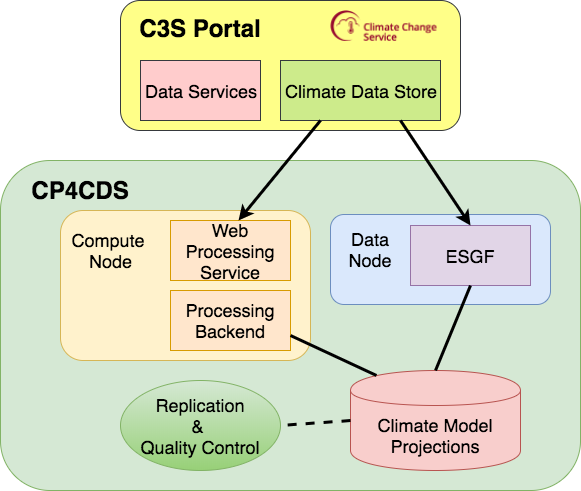
\includegraphics[width=0.8\linewidth]{cp4cds}
   \end{minipage}
   \begin{minipage}{0.6\textwidth}
     {\bf CP4CDS Overview}
     \begin{itemize}\compresslist
       \item Providing the required data and services for global climate projections
        to the {\bf Climate Data Store} (CDS) of the
        Climate Change Service (C3S) {\bf portal hosted at ECMWF, UK}
       \item Data Node - Consisting of vanilla {\bf Earth System Grid Federation} (ESGF) index and data node
       \item Compute Node - Providing compute facilities using the Web Processing Service (WPS) standard interface
       \item Processing Backend - {\bf External software toolbox} to analyse climate model projections
       \item Climate Model Projections (CMIP5, CORDEX) in filesystem cache
       \item Quality Control - {\bf Climate Model Projections} are selected for C3S and {\bf quality checked}
       \item Replication - Using {\bf Synda} Python library for managing data movement
     \end{itemize}
  \end{minipage}
  %\vspace{1em}

  \begin{minipage}{0.4\textwidth}
    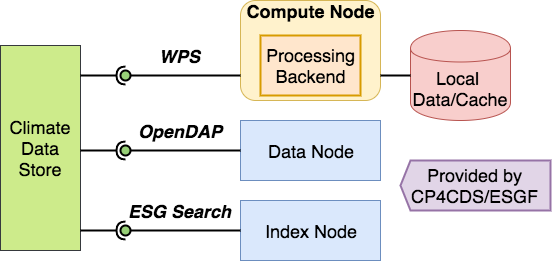
\includegraphics[width=0.8\linewidth]{cp4cds-interfaces}
  \end{minipage}
  \begin{minipage}{0.6\textwidth}
    {\bf Service Interfaces exposed to Climate Data Store (CDS)}
    \begin{itemize}\compresslist
      \item {\bf Web Processing Service} (WPS) - standard interface for processing
      \item OpenDAP - remote data access interface for NetCDF files
      \item ESG Search - adapted Solr search interface by ESGF for data discovery
    \end{itemize}
 \end{minipage}
 %\vspace{1em}

 \begin{minipage}{0.4\textwidth}
    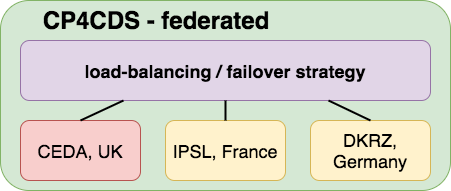
\includegraphics[width=0.8\linewidth]{cp4cds-federated}
  \end{minipage}
  \begin{minipage}{0.6\textwidth}
    {\bf Federated CP4CDS Nodes}
    \begin{itemize}\compresslist
      \item {\bf Geographically distributed and highly available} set of data and compute services
      \item Federated between the leading European institutes: CEDA, IPSL and DKRZ
      \item Using {\bf load-balancing across sites} / failover strategy
      %\item Data available at all 3 sites, replicas synchronised
      \item All 3 sites of the {\bf same replicated local data pool}
      \item All 3 sites have the {\bf same (exact version) software stack} using a common software deployment ({\bf SDDS})
      \item {\bf CEDA hosts the main node}, IPSL and DKRZ take over service when needed
    \end{itemize}
  \end{minipage}
  %\vspace{2em}
 }

%%%%%%%%%%%%%%%%%%%%%%%%%%%%%%%%%%%%%%%%%%%%%%%%%%%%%%%%%%%%%%%%%%%%%%%%%%%%%%
\headerbox{Architecture of Compute Node}{name=arch,column=1,span=2,below=cp4cds}{
%%%%%%%%%%%%%%%%%%%%%%%%%%%%%%%%%%%%%%%%%%%%%%%%%%%%%%%%%%%%%%%%%%%%%%%%%%%%%%
  \begin{minipage}{0.4\textwidth}
    \includegraphics[width=\linewidth]{cp4cds-wps}
  \end{minipage}
  \begin{minipage}{0.6\textwidth}
    {\bf Software Components of WPS Service}
    \begin{itemize}\compresslist
      \item A WPS request (HTTP GET/POST) comes from a WPS client.
      \item The {\bf Nginx/Gunicorn combination} delegates the request to the PyWPS WSGI application
      \item Gunicorn - spawns several workers to use the available CPUs on a single compute node
      \item {\bf PyWPS} - Python implementation of OGC Web Processing Standard
      \item Supervisor - used to start/stop and monitor services
      \item Processing outputs and status documents are web accessible by the Nginx file-service
      \item {\bf Token based access control} (using OAuth) for WPS service
      \item WPS Processes are defined for project analysis toolbox, like {\bf C3S MAGIC} diagnostics
      \item {\bf Processing Backend} has read-only access to the climate data pool on
        file-system with CMIP5 climate model projections and observational data.
      \item Using {\bf PyWPS scheduler extension} (Slurm, GridEngine) to run process on a compute-cluster for scalability
    \end{itemize}
  \end{minipage}
  %\vspace{1em}

  % \begin{minipage}{0.4\textwidth}
  %   \includegraphics[width=\linewidth]{pywps-scheduler-extension}
  % \end{minipage}
  % \begin{minipage}{0.6\textwidth}
  %   \begin{itemize}\compresslist
  %     \item PyWPS Scheduler Extension
  %   \end{itemize}
  % \end{minipage}

  % \begin{minipage}{0.4\textwidth}
  %   \includegraphics[width=0.2\linewidth]{conda}
  %   \includegraphics[width=0.1\linewidth]{ansible}
  %   \includegraphics[width=0.4\linewidth]{chaos}
  % \end{minipage}
  % \begin{minipage}{0.6\textwidth}
  %   \begin{itemize}\compresslist
  %     \item Using the Conda package manager to setup an environment with all used software components.
  %     \item Using Buildout/Ansible to setup a WPS (PyWPS) with all services (Supervisor, Gunicorn, Nginx)
  %       and configuration files.
  %     \item ``Managing the Chaos''
  %   \end{itemize}
  % \end{minipage}
  % \vspace{1em}

  % \begin{minipage}{0.4\textwidth}
  %   
\includegraphics[width=0.2\linewidth]{docker}
  %   \includegraphics[width=0.4\linewidth]{cp4cds-docker-cloud}
  % \end{minipage}
  % \begin{minipage}{0.6\textwidth}
  %   \begin{itemize}\compresslist
  %     \item A Dockerfile is generated using the Buildout setup for each WPS service
  %     \item Docker images are build automatically on Docker Cloud
  %   \end{itemize}
  % \end{minipage}
  % \vspace{1em}

  % \begin{minipage}{0.4\textwidth}
  %   \includegraphics[width=\linewidth]{esmvaltool}
  % \end{minipage}
  % \begin{minipage}{0.6\textwidth}
  %   \begin{itemize}\compresslist
  %     \item A community diagnostic and performance metrics tool for routine evaluation of Earth system models in CMIP
  %     \item Collection of diagnostics implemented in Python and NCL
  %   \end{itemize}
  % \end{minipage}
}

%%%%%%%%%%%%%%%%%%%%%%%%%%%%%%%%%%%%%%%%%%%%%%%%%%%%%%%%%%%%%%%%%%%%%%%%%%%%%%
\headerbox{Status}{name=status,column=1,span=2,below=arch}{
%%%%%%%%%%%%%%%%%%%%%%%%%%%%%%%%%%%%%%%%%%%%%%%%%%%%%%%%%%%%%%%%%%%%%%%%%%%%%%
  \begin{itemize}\compresslist
    \item A Copernicus WPS demo service is available on GitHub (CP4CDS repo)
    %\item A basic WPS template for SDDS is available on GiHub (CP4CDS repo)
    \item The new version of ESMValTool 2.x is used in CP4CDS via Conda package
    \item A PyWPS scheduler extension for Slurm and Grid-Engine was developed
    \item A security proxy for WPS services is available using X509 certificates and simple tokens
    \item A quality checked CMIP5 data store is available at CEDA and partly replicated to other sites
    %\item An inital ESGF node federation is set-up at all three CP4CDS sites
  \end{itemize}
}


%%%%%%%%%%%%%%%%%%%%%%%%%%%%%%%%%%%%%%%%%%%%%%%%%%%%%%%%%%%%%%%%%%%%%%%%%%%%%%
\headerbox{C3S MAGIC - Climate Data Analysis}{name=magic,column=3,span=1}{
%%%%%%%%%%%%%%%%%%%%%%%%%%%%%%%%%%%%%%%%%%%%%%%%%%%%%%%%%%%%%%%%%%%%%%%%%%%%%%
  \center
  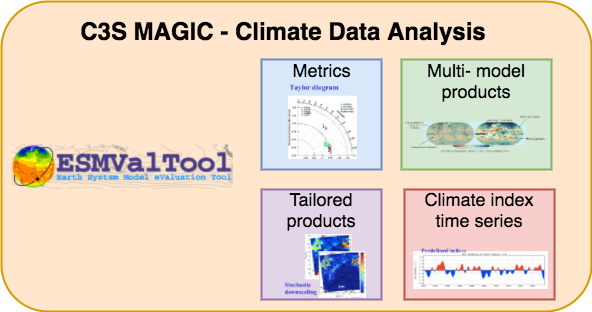
\includegraphics[width=0.7\linewidth]{c3s-magic}

    %{\bf C3S MAGIC - data manipulation and analysis package}
    \begin{itemize}\compresslist
      \item {\bf C3S MAGIC} - data manipulation and analysis package
      \item {\bf Developed by KNMI, eScience Center, DLR} and others
      \item Used by CP4CDS as {\bf Processing Backend} for CMIP5 climate model projections
      \item To {\bf calculate standardized characteristics}
          %(metrics, statistics, time series)
          from available climate model output
      %\item some of these characteristics are pre-defined, while others require user input
      \item {\bf ESMValTool} - To develop and deliver an enhanced version of the ESMValTool software
      \item {\bf Metrics} - computes and displays a wide set of performance metrics and diagnostics
        %relevant for sectoral information services
      \item {\bf Multi-model products} - To combine the climate information generated by various climate models
        into a single estimate of any future climate signal
        %that is optimally suited to provide the requested (sectoral) climate change information
      \item {\bf Climate index time-series} - To compute single-model and multi-model time series of climate indices
        %for both pre-defined indices and indices defined interactively by the user
      \item {\bf Tailored products} - To assure that specific needs of envisaged end users in the selected economic
        sectors
        %(energy, insurance, water/hydrology and coastal areas)
        are facilitated by the software
    \end{itemize}

}

%%%%%%%%%%%%%%%%%%%%%%%%%%%%%%%%%%%%%%%%%%%%%%%%%%%%%%%%%%%%%%%%%%%%%%%%%%%%%%
\headerbox{SDDS - Deployment Solution}{name=sdds,column=3,span=1,below=magic}{
%%%%%%%%%%%%%%%%%%%%%%%%%%%%%%%%%%%%%%%%%%%%%%%%%%%%%%%%%%%%%%%%%%%%%%%%%%%%%%

  \center
  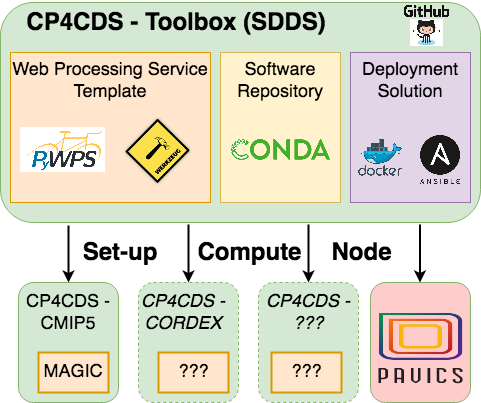
\includegraphics[width=0.7\linewidth]{cp4cds-toolbox}

    %{\bf Manage and deploy Software for CP4CDS Compute Nodes}
    \begin{itemize}\compresslist
      \item {\bf SDDS} - Software Deployment and Dependency Solution
      \item To {\bf manage and deploy codes} from external projects,
        such as {\bf C3S MAGIC / ESMValTool}, into the CP4CDS Compute Node
      \item Consists of a software environment and application, {\bf managed through a GitHub repository},
        which includes {\bf a basic template of a working WPS service} (PyWPS)
      \item {\bf Conda} -  The template uses a Conda ``environment'' to record the software dependencies
        % and to build a reproducible software installation
      \item {\bf Docker} - Used to provide the Compute Node through containers
      \item {\bf Ansible} - Ansible is used to setup a WPS (PyWPS) % with all services
        % (Supervisor, Gunicorn, Nginx) and configuration files
      % \item SDDS is used to set-up CP4CDS Compute Nodes for CMIP5 (global) and CORDEX (regional) climate projections with
      %   a specific analysis toolbox
    \end{itemize}

}

%%%%%%%%%%%%%%%%%%%%%%%%%%%%%%%%%%%%%%%%%%%%%%%%%%%%%%%%%%%%%%%%%%%%%%%%%%%%%%
\headerbox{Next Steps}{name=next,column=3,span=1,below=sdds}{
%%%%%%%%%%%%%%%%%%%%%%%%%%%%%%%%%%%%%%%%%%%%%%%%%%%%%%%%%%%%%%%%%%%%%%%%%%%%%%
  % \begin{itemize}\compresslist
  %   \item C3S overview and C3S Climate Data Store (CDS)
  %   \item The CP4CDS project overview: ESGF Data Nodes, Index Nodes and CP4CDS Compute Nodes,
  %     load-balancing across sites, QC'd CMIP5 data.
  %   \item Requirement to deploy code from other projects/groups into the CP4CDS Compute Node, such as ESMValTool.
  %   \item Chosen technology: Birdhouse WPS environment
  %   \item Why Birdhouse? python, open source, actively developed, good design, client/security components, PyWPS extensions.
  %   \item SDDS/Compute Node overview: including PyWPS cluster configuration for scalability.
  %   \item SDDS workflow: template, GitHub fork etc
  %   \item Status and next steps
  % \end{itemize}
  \begin{itemize}\compresslist
    %\item A PyWPS scheduler extension to use a Docker container for each process execution request is planned
    %\item Implementing the latest WPS 2.0.0 standard in PyWPS (WPS 1.0.0 + job-cancel funtion
    \item Further integration of MAGIC codes
    \item Roll-out of CP4CDS at all three sites
    \item Improved SDDS - using a template generator, replacing Buildout by Ansible, deployment in Docker Cluster
    \item Using ESGF OAuth service for security tokens
    \vspace{0.5em}
  \end{itemize}
}

\end{poster}

\end{document}
